\chapter{Semantics}
\label{semanticschapter}

\section{Introduction}

The purpose of this chapter is to describe how the semantics of
modelling and programming languages can be described using
metamodels. The semantics of a modelling language describes what
the language means in terms of its behaviour, static properties or
translation to another a language. The chapter begins by
motivating the need for semantics and then describes a number of
different approaches to defining semantics using metamodels. These
approaches aim to provide a way of constructing platform
independent models of semantics - thus enabling the semantics of a
language to be interchanged between metamodelling tools.  An
example of how the approaches can be used to define the semantics
of the StateMachine language is then presented.

\section{What is Semantics?}

In general terms, a language semantics describes the {\em meaning}
of concepts in a language. When using a language, we need to
assign a meaning to the concepts in the language if we are to
understand how to use it. For example, in the context of a
modelling language, our understanding of the meaning of a
StateMachine or the meaning of a Class will form a key part of how
we choose to use them to model a specific aspect of a problem
domain.

There are many ways of describing meaning of a language concept.
Consider the ways in which the meaning of concepts in natural
languages can be described:

\begin{itemize}
\item In terms of concepts which already have a well defined
meaning. For instance "a car consists of a chassis, four wheels,
an engine, body, and so on". This is only meaningful if the
concepts themselves are well defined. \item By describing the
properties and behaviour of the concept: "a car can be stationary,
or can be moving, and pressing the accelerator increases its
speed". \item As a specialisation of another concept. For
instance, "a truck is a vehicle with a trailer". \item By
describing the commonly shared properies of all possible instances
of a concept. For example, the concept of a car could be described
in terms of the valid properties that every instance of a car
should have.
\end{itemize}

In a natural language, semantics is a correlation or mapping
between concepts in a language with thoughts and experiences of
concepts in world around us. Although a more formal approach to
semantics is required for modelling and programming languages,
there is a close parallel to the approaches used to express
natural language semantics described above. In both cases, a key
requirement of a semantics is that it should be of practical use
in understanding the meaning of a language.

\section{Why Semantics?}

A semantics is essential to communicate the meaning of models or
programs to stakeholders in the development process. Semantics
have a central role to play in defining the semantically rich
language capabilities such as execution, analysis and
transformation that are required to support Language-Driven
Development. For example, a language that supports behaviour, such
as a StateMachine, requires a semantics in order to describe how
models or programs written in the language execute.

Traditionally, the semantics of many modelling languages are
described in an informal manner, either through natural language
descriptions or examples. For instance, much of the UML 1.X
specification \cite{umlspec} makes use of natural language
descriptions of semantics.

However, an informal semantics brings with it some significant problems:

\begin{itemize}
\item Because users have to assign an informal or intuitive
meaning to models, there is significant risk of misinterpretation
and therefore misuse by the users of the modelling language.

\item An informal semantics cannot be interpreted or understood by tools. Tool
builders are thus required to implement their own interpretation
of the semantics. Unfortunately, this means that the same language
is likely to be implemented in different ways. Thus, two different
tools may offer contradictory implementations of the same
semantics, e.g. the same StateMachine may execute differently
depending on the tool being used!

\item An informal semantics makes the task of defining new
languages difficult. It  makes it hard to identify areas where
concepts in the languages are semantically equivalent or where
there are contradictions. It is harder still to extend an existing
language if the semantics of the language are not defined.

\item Standards require precise semantics. Without them, a
standard is open to misunderstanding and misuse by practitioners
and tool developers while significantly limiting interoperablity.
\end{itemize}

\section{Semantics and Metamodels}

While it is clear that semantics is crucial part of a language
definition, the question is how should semantics be described? One
approach is to express semantics in terms of a formal,
mathematical language. Many academic papers have been written
describing the semantics of modelling languages in this way. Yet,
the complex mathematical descriptions that result are hard to
understand and are of limited practical use. Another approach is
to express semantics in terms of an external programming language.
This is a far more practical solution. Nevertheless, it results in
a definition which is tied to a specific programming language thus
compromising its platform independence. Furthermore, being forced
to step out of the metamodelling environment into a programming
language makes for a very non-intuitive language definition
process.

An alternative strategy is to describe the semantics of languages
using metamodels. There are some significant benefits to this
approach. Firstly, the semantics of a language is fully integrated
in the language's definition, which means the task of relating it
to other language design artifacts (concrete syntax, mappings,
abstract syntax, etc) is immediately simplified. Secondly, because
the same metamodelling language is used across all languages,
semantic definitions become reusable assets that can be integrated
and extended with relative ease. Finally, and most crucially,
semantics definitions are platform independent - they can be
interchanged in the same way, and if they are understood by the
tool that imports them, they can be used to drive the way that the
tool interacts with the language. For instance, a semantics that
describes how a StateMachine executes can be used to drive
simulators across a suite of compliant tools. The ability to
define semantics in a platform independent way is crucial to the
success of Language-Driven Development. It enables tools to be
constructed for languages that are both portable and interoperable
irrespective of the environment in which they are defined.

It is important to note that a metamodel semantics is quite
different  from the abstract syntax model of a language, which
defines the structure of the language. However, an abstract syntax
model is a pre-requisite for defining a semantics, as a semantics
adds a layer of meaning to the concepts defined in the abstract
syntax. Semantics in this sense should also be distinguished from
static semantics, which are the rules which dictate whether or not
an expression of the language is well-formed. Static semantics
rules are those employed by tools such as type checkers.

\section{Approaches}

There are many different approaches to describing the semantics of
languages in a metamodel. This section examines some key
approaches and gives examples of their application. All the
approaches are motivated by approaches to defining semantics that
have widely been applied in programming language domains. The main
difference is that metamodels are used to express the semantic
definitions.

The approaches include:

\begin{description}
\item [Translational] Translating from concepts in one language
into concepts in another language that have a precise semantics.
\item [Operational] Modelling the operational behaviour of
language concepts. \item [Extensional] Extending the semantics of
existing language concepts.\item [Denotational] Modelling the
mapping to semantic domain concepts.

\end{description}

Each approach has its own advantages and disadvantages. In
practice, a combination of approaches is typically used, based on
the nature of individual concepts in the language. In each case,
it is important to note that the semantics are described in the
metamodelling language - no external formal representation is
used. The following sections describe each of the approaches,
along with a small example of their application.

\section{Translational Semantics}

Translational semantics is based on two notions:

\begin{itemize}
\item The semantics of a language is defined when the language is
translated into another form, called the target language. \item
The target language can be defined by a small number of primitive
constructs that have a well defined semantics.
\end{itemize}

The intention of the translational approach is to define the
meaning  of a language in terms of primitive concepts that have
their own well defined semantics. Typically, these primitive
concepts will have an operational semantics (see later).

The advantage of the translational approach is that provided there
there is a machine that can execute the target language, it is
possible to directly obtain an executable semantics for the
language via the translation. This approach is closely related to
the role played by a compiler in implementing a richer programming
language in terms of more primitive executable primitives.

The main disadvantage of the approach is that information is lost
during the transformation process. While the end result is a
collection of primitives, it will not be obvious how they are
related to the original modelling language concepts. There are
ways to avoid this, for instance information about the original
language concepts can be "tagged" onto the target language, thus
enabling it to retain information about the structure of the
original language. Alternatively, one may consider maintaining
information about the mapping between the two models.

The translational approach can be incorporated in a language
definition in many different ways:

\begin{itemize}
\item Within a language metamodel by translating one concept into
a concept that has a semantics, e.g. translating a case statement
into a sequence of if statements, where the if statements have an
operational semantics. Another example might be translating a rich
mapping language into a collection of primitive mapping functions
with additional information tagged onto the primitives to indicate
the structure of the source language. \item Between language
metamodels, by translating one metamodel into another. For
example, an abstract syntax metamodel for UML can be mapped to a
metamodel of a small well-defined language such as XCore, or to a
programming language such as Java.
\end{itemize}

\subsection{Approaches}

There are a number of different approaches to implementing a
transformational semantics in XMF:

\begin{itemize}
\item A mapping can be defined between the abstract syntax of the
source and target languages. This could be written in a mapping
language (such as XMap), or implemented by appropriate operations
on the source model. \item The result of parsing the concrete
syntax of the source language can be used to directly create an
instance of the target language. \item The result of parsing the
concrete syntax can be translated directly into machine code that
can be run on the XMF virtual machine.
\end{itemize}

In the second approach, the intermediate step of generating an
abstract syntax model for the source language can be omitted. The
concrete syntax of the source language thus acts as {\em sugar}
for the target language. This approach is particularly useful when
constructing new types of expressions that can be desugared into a
number of more primitive concepts, e.g. translating a case
statement into a collection of if expressions.

The third approach requires the construction of machine code
statements but has the advantage of resulting in a highly
efficient implementation.

\subsection{Example}

Because XMF provides a number of well defined primitives, it is a
good target for translation. As an example, consider defining a
semantics for StateMachines via a translation from the
StateMachine abstract syntax model (described in chapter
\ref{abschapter}). The mapping language used in this example is
described in detail in chapter \ref{mappingchapter}.  A summary of
the approach taken is shown in figure \ref{translationExample}.

\begin{figure}[htb]
\begin{center}
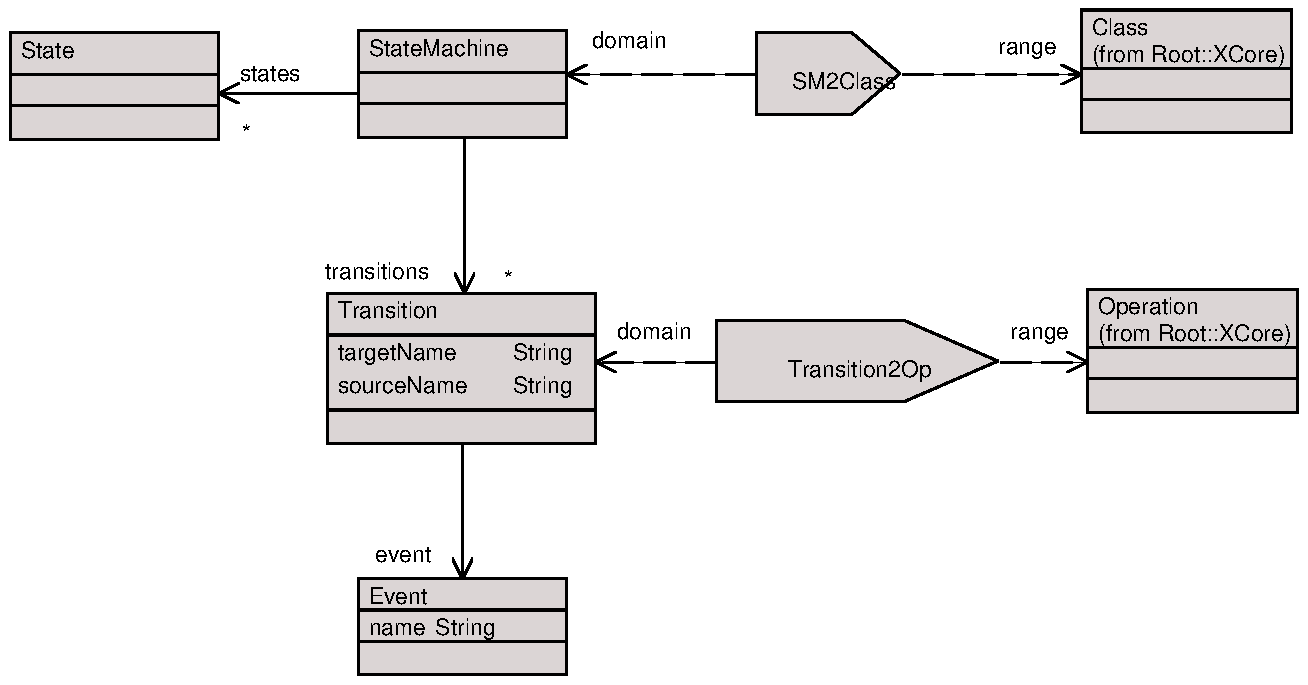
\includegraphics[width=14cm]{Semantics/figures/Translational.pdf}
\caption{Overview of the translational mapping example}
\label{translationExample}
\end{center}
\end{figure}

The aim is to translate a StateMachine into an instance of a XCore
Class such that semantics of the StateMachine is preserved. This
is achieved by ensuring that the Class simulates the behaviour of
the StateMachine:

\begin{itemize}
\item The StateMachine is translated into a Class containing an
attribute called {\em state}, whose permitted values are the
enumerated state names of the StateMachine.
\item The Class will inherit all the attributes and operations
of the StateMachine's context class.
\item Each transition of the StateMachine is translated
into an operation of the Class with the same name as the
transition's event.
\item The transition will contain code that will simulate the
invocation of the transition's guard and actions, causing the value
of {\em state} to change.
\end{itemize}

\noindent The following pattern of code will thus be required in
the body of each operation:

\begin{lstlisting}
  if <guard> then
    self.state := <target-state-name>;
    <action>
  end
\end{lstlisting}

Where $<$guard$>$ and $<$action$>$ are the bodies of the
corresponding transition's guard and action, and
$<$target-state-name$>$ is the name of the state that is the target
of the transition.

The most challenging part of this translation is creating the
appropriate code bodies in each operation. The following code
shows how XOCL can be used to define an operation, transitionOp(),
which given the guard, action, event name and target name of a
transition, returns an XCore operation that simulates the
transition. This operation is called by the transition2Op mapping.
Note that in the operation transitionOp() an operation cannot be
assigned a name until it is declared, thus setName() is used to
assign it a name after it has been declared.

\begin{lstlisting}
@Map Transition2Op
  @Operation
  transitionOp(g:Operation,a:Operation,eventName,targetName)
    let op = @Operation()
      if g() then
        a();
        self.state := targetName
      end
    end
    in
      op.setName(eventName);
      op
    end
  end

  @Clause Transition2Op
    Transition
      [event = Set{
        Event
          [name = N]
        },
       name = T,
       guard = G,
       action = A]
    do
      self.transitionOp(G,A,N,T.name)
  end
end
\end{lstlisting}

This definition of transitionOp() makes use of the fact that in
XMF an Operation is also an Object and can therefore be assigned
to a variable.

As an example, consider the simple traffic light model shown in
figure \ref{trafficlight}. The result of applying the
Transition2Op mapping to the GreenRed() transition will be the
following XOCL operation:

\begin{figure}[htb]
\begin{center}
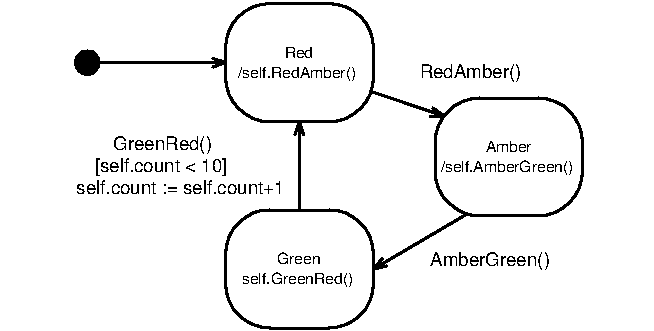
\includegraphics[width=11cm]{Semantics/figures/trafficlight.pdf}
\caption{The traffic light example} \label{trafficlight}
\end{center}
\end{figure}

\begin{lstlisting}
@Operation GreenRed()
  if g() then
    a();
    self.state := "Red"
  end
end
\end{lstlisting}

\noindent where g and a are the following anonymous operation
definitions:

\begin{lstlisting}
@Operation anonymous()
 self.count < 10
end

@Operation anonymous()
  self.count := self.count + 1
end
\end{lstlisting}

\section{Operational Semantics}

An operational semantics describes how models or programs written
in a language can be directly executed. This involves constructing
an interpreter. For example, an assignment statement �V := E� can
be described by an interpreter that executes the steps that it
performs: Evaluate the expression E and then change the value
bound to the variable V to be the result.

The advantage of an operational semantics is that it is expressed
in terms of operations on the language itself. In contrast, a
translational semantics is defined in terms of another, possibly
very different, language. As a result, an operational semantics
can be easier to understand and write.

Writing an interpreter as part of a metamodel relies on the
metamodelling language itself being executable. Provided this is
the case, concepts can define operations that capture their
operational behaviour.

Typically, the definition of an interpreter for a language follows
a pattern in which concepts are associated with an operational
description as follows:

\begin{itemize}
\item Operations will be defined on concepts that implement their
operational semantics e.g. an action may have an run() operation
that causes a state change, while an expression may have an eval()
operation that will evaluate the expression. \item The operations
typically take an environment as a parameter: a collection of
variable bindings which will be used in the evaluation of the
concepts behaviour, and a target object, which will be the object
that is changed as a result of the action or which represents the
context of the evaluation. \item The operations will return the
result of the evaluation (a boolean in the case of a static
expression) or change the value of the target object (in the case
of an action).
\end{itemize}

\subsection{Example}

A StateMachine can be given an operational semantics by defining
an interpreter that executes a StateMachine. It is implemented by
constructing a run() operation for the StateMachine class. We also
add an attribute messages, which records the messages that are
pending on the StateMachine as a result of a send action on a
transition:

\begin{figure}[htb]
\begin{center}
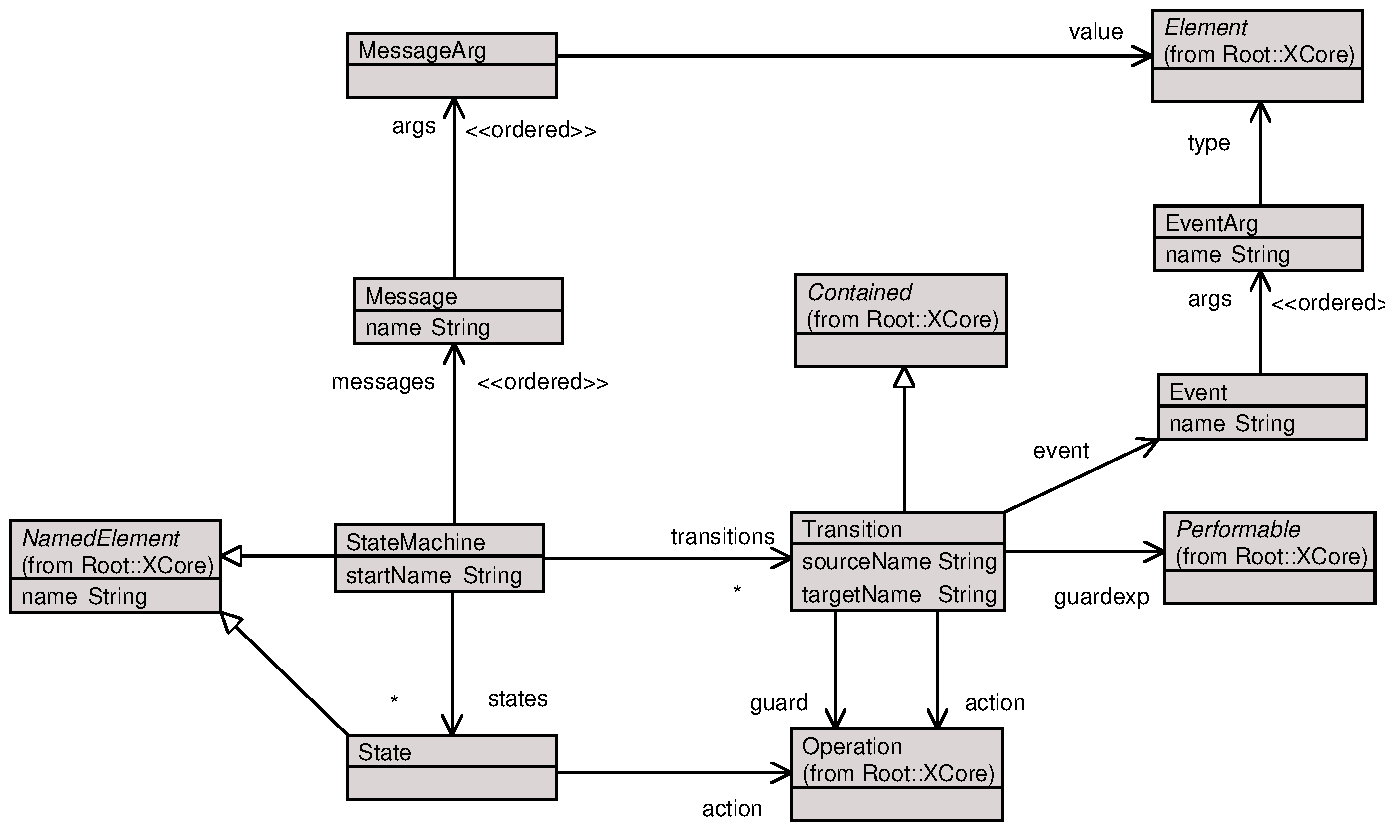
\includegraphics[width=15cm]{Semantics/figures/messages.pdf}
\caption{StateMachine model extended with message queues}
\label{messages}
\end{center}
\end{figure}

\noindent The code that executes the run() operation is below.
More details about the executable language used here, and the use
of executability as a means of defining semantics, will be
explained in chapter \ref{execChapter}.

\begin{lstlisting}
@Operation run(element)
      let state = self.startingState() in
        @While state <> null do
          let result = state.activate(element) then
            transitions = self.transitionsFrom(state) then
            enabledTransitions = transitions->select(t |
            t.isEnabled(element,result) and
            if t.event <> null then
              messages->head().name = t.event.name
            else
              true
            end) in
              if enabledTransitions->isEmpty then
                state := null
              else
              let transition = enabledTransitions->sel in
                transition.activate(element,result + self.messages->head().args.value);
                state := transition.target();
                if transition.event <> null then
                  self.messages := self.messages->tail()
                end
              end
            end
          end
        end
      end
    end
\end{lstlisting}

The operation takes the element that the StateMachine is being
applied to. It first sets the state to be the starting state,
then enters a while loop. Provided that the StateMachine has not
terminated (state $<>$ null) the following is peformed:

\begin{enumerate}
\item The entry action on the current state is invoked by calling
its activate operation. \item The collection of enabled
transitions is determined by selecting all the transitions that
leave the current state such that the evaluation of their guard is
true, and that an event is waiting on the machine that corresponds
to the event on the transition. \item If there are no enabled
transitions, the state is set to null, and the run() operation
terminates. \item If there are enabled transitions, one of them is
chosen and its action is invoked, before assigning the state to be
the target of the transition.
\end{enumerate}

Consider the traffic light example shown in figure
\ref{trafficlight}. If the current state of the StateMachine is
Green, then the above semantics ensures that the guard on the
GreenRed() transition will be evaluated and if it returns true the
action on transition will be executed.

As this example shows, complex behaviour can be captured in terms
of operational definitions. Moreover, the definition can
immediately be tested and used within a tool to provide
semantically rich means of validating and exercising models and
programs written in the language.

\section{Extensional Semantics}

In the extensional approach, the semantics of a language is
defined as an extension to another language. Modelling concepts in
the new language inherit their semantics from concepts in the
other language. In addition, they may also extend the semantics,
adding new capabilities for example.

The benefit of the approach is that complex semantic concepts can
be reused with minimum effort. For example, a business entity need
not define what it means to create new instances, but can inherit
the capability from Class.

The extensional approach has some commonality with the notion of a
profile (\cite{umlspec}). A profile provides a collection of
stereotypes, which can be viewed as sub-classes of UML or MOF
model elements. However, by performing the extension at the
metamodel level, greater expressibility is provided to the user,
who can add arbitrarily rich semantic extensions to the new
concept. A suitable tool can make use of this information to
permit the rapid implementation of new modelling languages. It may
recognise that an extension has occurred, and use stereotype
symbols to tailor the symbols of the original modelling language
to support the new language (see section \ref{stereotypes}).

\subsection{Example}

As an example, consider the requirement to be able to create
multiple instances of the same StateMachine. This can be achieved
by specialising the class Class from the XCore metamodel (see
figure \ref{extensionExample}. Because Class is instantiable, the
StateMachine will also inherit its semantics.

\begin{figure}[htb]
\begin{center}
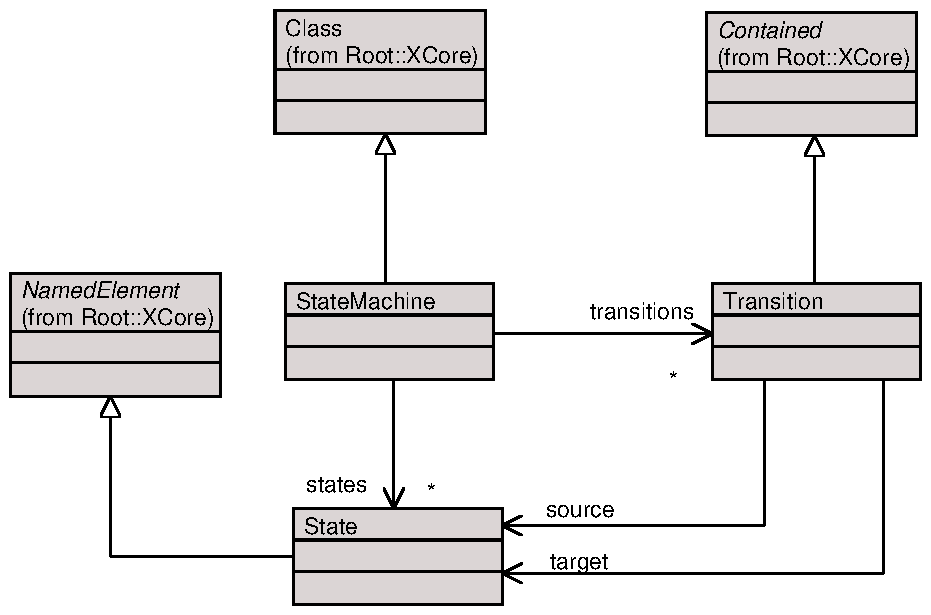
\includegraphics[width=11cm]{Semantics/figures/extension.pdf}
\caption{Example of extending the class Class}
\label{extensionExample}
\end{center}
\end{figure}

By specialising the class NamedElement a State can be owned by a
StateMachine and can be navigated to via a pathname. Similarly, a
Transition can owned by a StateMachine, but in this case it cannot
have a name as it specialises the class Contained.

While the extensional approach is appealing in terms of its
simplicity, it does have its disadvantages. Firstly, it is
tempting to try and 'shoe-horn' the complete semantics of a
language into this form. In practice this is usually not possible
as there will be concepts that simply do not fit. In these cases,
other approaches to defining semantics must be used.

\section{Denotational Semantics}

The purpose of denotational semantics is to associate mathematical
objects, such as numbers, tuples, or functions, with each concept
of the language. The concept is/are said to {\em denote} the
mathematical object(s), and the object is called the {\em
denotation} of the concept. The objects associated with the
concept are said to be the {\em semantic domain} of the concept. A
widely used example of this in programming language semantics is
the denotation of the operation + by a number. For instance, the
denotation of 4+5 is 9.

A denotational semantics can be thought of as semantics by
example. By providing all possible examples of a concept's
meaning, it is possible to define precisely what it means. In the
above example, there is only one denotation. However, many
concepts are denoted by a collection of examples. To describe the
semantics of an Integer, the set of all positive numbers would be
required, i.e. the denotation of Integer is 0..infinity.
Denotational descriptions of semantics tend to be static, i.e.
they enumerate valid instances of a concepts, and a non-executable
fashion.

Here are some common examples of denotational relationships found
in metamodels:

\begin{itemize}
\item The denotation of a Class is the collection of all Objects
that may be an instance of it. \item The denotation of an Action
is a collection of all possible state changes that can result from
its invocation. \item The denotation of an Expression is the
collection of all possible results that can be obtained from
evaluating the expression.
\end{itemize}

A denotational semantics can be defined in a metamodel by
constructing a model of the language's abstract syntax and
semantic domain and of the semantic mapping that relates them.
Constraints are then written that describe when instances of
semantic domain concepts are valid with respect to their abstract
syntax. For example, constraints can be written that state when an
Object is a valid instance of a Class.

The advantage of the denotational approach is its declarative
nature. In particular, it captures semantics in a way that does
not commit to a specific choice of operational semantics. For
instance, while an operational semantics would have to describe
how an expression is evaluated, a denotational semantics simply
describes what the valid evaluation/s of the expression would be.

In practice a purely denotational approach is best used when a
high-level specification of semantics is required. It is
particularly useful in a standard where commitment to a specific
implementation is to be avoided. Because they provide a
specification of semantics they can be used to test
implementations of the standard: candidate instances generated by
an implementation can be checked against the denotational
constraints. A good example of the denotational semantics approach
is the OCL 2.0 specification \cite{ocl2}, where they are used to
describe the semantics of OCL expressions.

\subsection{Example}

We can describe the execution semantics of a StateMachine by
modelling the semantic domain concepts that give it a meaning. A
useful way of identifying these concepts is to consider the
vocabulary of concepts we would use to describe the behaviour of a
StateMachine. This might include concepts such as a state change
(caused by a transition), examples of statemachines in specific
states, and message queues.

Figure \ref{sdExample} shows an example of a semantic domain that
might result from generalising these concepts into a model.

\begin{figure}[htb]
\begin{center}
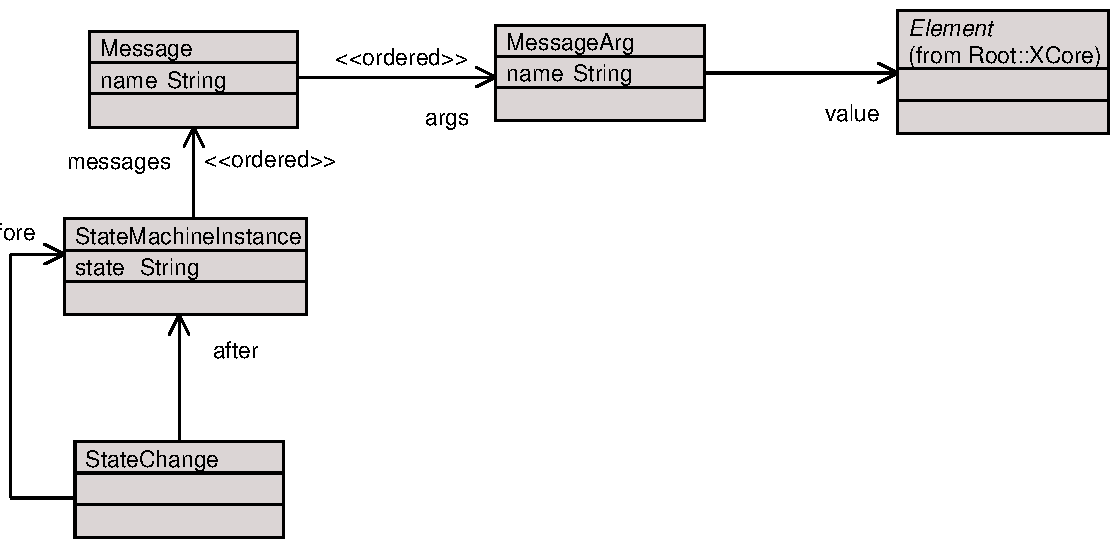
\includegraphics[width=14cm]{Semantics/figures/semanticdomain.pdf}
\caption{A semantic domain for StateMachines} \label{sdExample}
\end{center}
\end{figure}

The denotation of a StateMachine is essentially a model of the
valid state changes that may occur to the StateMachine at any
point in time. Here a StateMachineInstance is used to model a
StateMachine at a specific point in time. It has a state, and a
sequence of messages which are waiting to be consumed by the
machine. State changes represent the invocation of a transition,
causing the StateMachine to move from one state (the before state)
to another (the after state).

Using this model, many different examples of valid StateMachine
behaviours can be tested. The snapshot in figure \ref{sdsnapshot}
shows a fragment of the behaviour of a machine that has two
transitions from the state A to the state B and back again.

\begin{figure}[htb]
\begin{center}
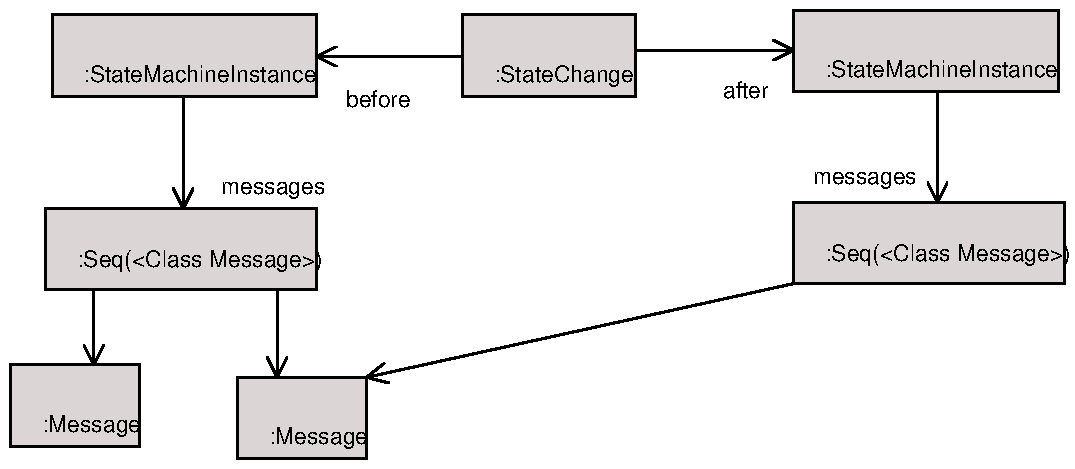
\includegraphics[width=13cm]{Semantics/figures/sdsnapshot.pdf}
\caption{An example snapshot of a StateMachine's behaviour}
\label{sdsnapshot}
\end{center}
\end{figure}

In order to complete the model, the relationship between the
semantic domain and abstract syntax model must also be modelled.
This relationship, commonly called a {\em semantic mapping}, is
crucial to defining the semantics of the language. It makes
precise the rules that say when instances of semantic domain
concepts are valid with respect to a abstract syntax model. In
this case, when a particular sequence of state changes is valid
with respect to a specific StateMachine.

Figure \ref{semanticmapping} shows the semantic mapping model. A
StateMachineInstance is associated with its StateMachine, while a
StateChange and Message are associated with the Transition and
Event that they are instances of.

\begin{figure}[htb]
\begin{center}
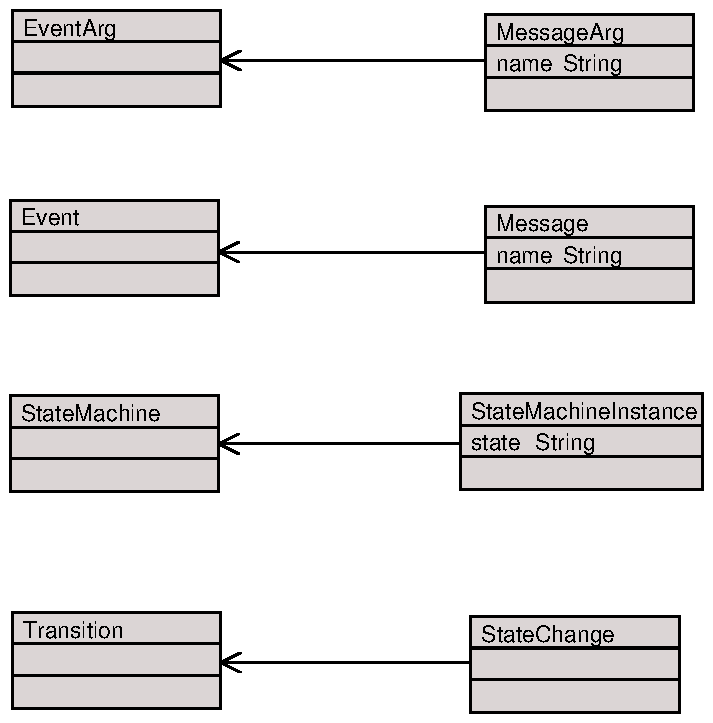
\includegraphics[width=8cm]{Semantics/figures/semanticmapping.pdf}
\caption{Semantic mapping model for the StateMachine language}
\label{semanticmapping}
\end{center}
\end{figure}

Finally, well-formedness rules will be required. An example is the
rule which guarantees that the before and after states of a
StateChange commutes with the source and target states of the
transition it is an instance of:

\begin{lstlisting}
context StateChange
  self.transition.sourceName = self.before.state.name and
  self.transition.targetName = self.after.state.name
\end{lstlisting}

Other rules will be required to ensure that the state changes
associated with a state machine are valid with respect to its
execution semantics. These will describe such aspects as the
conditions under which transitions are enabled, and the order in
which they may fire.

\section{Process}

The choice of semantics depends on the type of language being
defined. The following pointers provide a guide to choosing the
most appropriate approach.

\begin{itemize}
\item If a declarative, non executable semantics is required, use
the denotational approach. \item If a language has concepts that
need to be evaluated, executed or instantiated then they should be
modelled using an operational, translational or extensional
approach. The choice of approach will be based on the following:
  \begin{itemize}
  \item If a concept is clearly a sugared form of more primitive
  concepts, adopt a translation approach. This avoids having to
  construct a semantics for the concept from scratch - reuse the
  semantic machinery that has already been defined for the primitive
  concepts. This approach should only be used when it is
  acceptable to loose information about the original concept.
  \item If information must be kept about the concept and it is
  possible to reuse an existing concept use the extensional approach.
  \item If there is no convenient means of reusing an existing
  concept use the operational approach to construct an interpreter.
  \end{itemize}
\end{itemize}

Note, there are no hard and fast rules to choosing an approach.
The primary aim should be to develop a semantic model that meets
the needs of the stakeholders of the language.

\section{Conclusion}

Semantics is crucial in being able to understand the meaning of a
modelling language, to be able to interact with it a meaningful
way, and to be able to support truly interoperable language
definitions. This chapter has shown that a language semantics can
be successfully captured with a metamodel. The key advantages are
that the semantics becomes an integrated part of the language
definition while remaining understandable to users and modelling
tools.
